\documentclass[dvipdfmx]{beamer}
\usetheme[
    block=fill, % ブロックに背景をつける
    progressbar=foot, % 各スライドの下にプログレスバー
    numbering=fraction % 合計ページ数を表示
]{metropolis}           % Use metropolis theme
\usepackage{float}
\usepackage{booktabs}
\usepackage{ascmac}
\usepackage{fancybox}
\usepackage{amsmath}
\usepackage{mathtools}
\renewcommand{\kanjifamilydefault}{\gtdefault} % 和文デフォルトをゴシック体に
\usecolortheme{rose}
\usepackage{tikz}
\usetikzlibrary {arrows.meta}
\usetikzlibrary {bending}
\usepackage{listings,jvlisting} %日本語のコメントアウトをする場合jvlisting(もしくはjlisting)が必要
%ここからソースコードの表示に関する設定
\lstset{
  basicstyle={\ttfamily},
  identifierstyle={\small},
  commentstyle={\smallitshape},
  keywordstyle={\small\bfseries},
  ndkeywordstyle={\small},
  stringstyle={\small\ttfamily},
  frame={tb},
  breaklines=true,
  columns=[l]{fullflexible},
  numbers=left,
  xrightmargin=0zw,
  xleftmargin=3zw,
  numberstyle={\scriptsize},
  stepnumber=1,
  numbersep=1zw,
  lineskip=-0.5ex
}

\title{進捗報告}
\date{\today}
\author{水野泰旭}
\institute{弘前大学理工学部電子情報工学科4年}
\subject{学習率による正解率向上}
\begin{document}
  \maketitle
  
  \begin{frame}
    \begin{block}{Deep\_Conv①\footnote{活性化関数はReluを使用}}
      \begin{enumerate}
        \item 畳み込み層\mbox{} (16, ((3, 3)))
        \item MAXプーリング\mbox{} ((2, 2))
        \item 畳み込み層\mbox{} (16, ((3, 3)))
        \item MAXプーリング\mbox{} ((2, 2))
        \item 畳み込み層\mbox{} (16, ((3, 3)))
        \item MAXプーリング\mbox{} ((2, 2))
        \item 畳み込み層\mbox{} (16, ((3, 3)))
        \item MAXプーリング\mbox{} ((2, 2))
      \end{enumerate}
    \end{block}
  \end{frame}

  \begin{frame}
    \begin{block}{Deep\_Conv①\footnote{活性化関数はReluを使用}}
      \begin{enumerate}
        \item Flatten層
        \item ドロップアウト層\mbox{} (ドロップアウト率0.3)
        \item 全結合層\mbox{} (64)
        \item ドロップアウト層\mbox{} (ドロップアウト率0.3)
        \item 全結合層(64)\mbox{}
        \item 出力層\mbox{} (5, 'softmax')
      \end{enumerate}
    \end{block}
  \end{frame}

  \begin{frame}
    Test Accuracy: 0.949519
    \begin{figure}[H]
      \centering  
      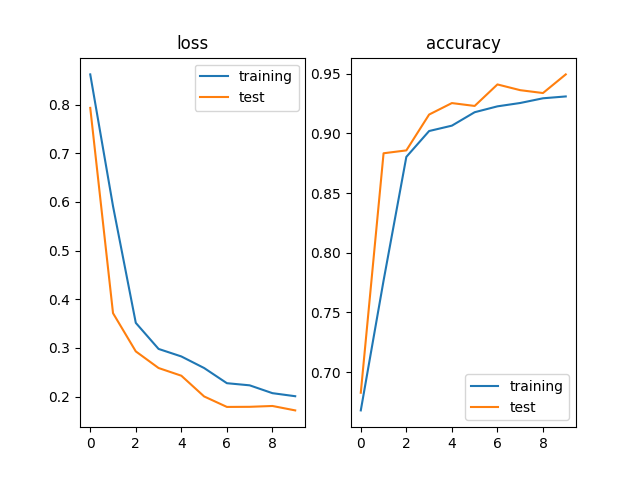
\includegraphics[keepaspectratio, scale=.55]{images/train_deep_conv_lr0.01.png}
      \caption{学習率0.01}
      \label{deep_conv_lr=0.01}
    \end{figure}
  \end{frame}

  \begin{frame}
    Test Accuracy: 0.956730
    \begin{figure}[H]
      \centering  
      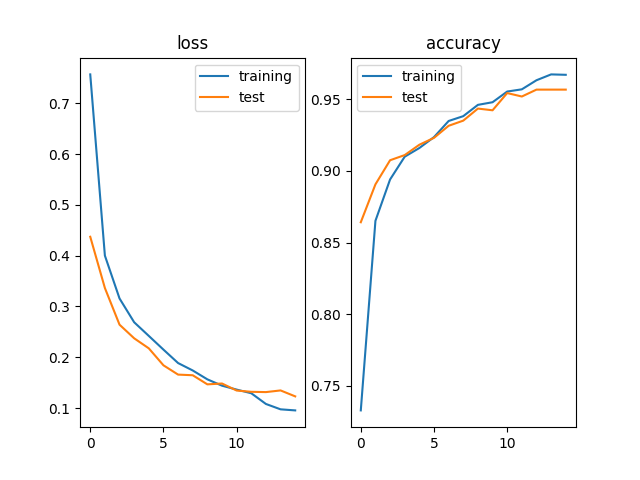
\includegraphics[keepaspectratio, scale=.55]{images/train_deep_conv_lr0.001.png}
      \caption{学習率0.001}
      \label{deep_conv_lr=0.001}
    \end{figure}
  \end{frame}

  \begin{frame}{これから取り組むこと}
    \begin{itemize}
      \item ハイパーパラメータの調節
      \item 交差検証
      \item 間違えた画像を調べる
    \end{itemize}
  \end{frame}

\end{document}


